% A basis open set U x V of the product [0,1] x [0,1].
% Source: book/tex/topology/constructions.tex (§ Product topology).
\documentclass[border=2mm]{standalone}
\usepackage{tikz}
\begin{document}
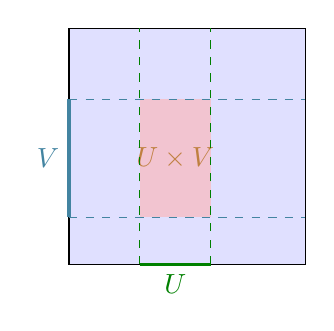
\begin{tikzpicture}[scale=3]
  \fill[blue!12] (0,0) rectangle (1,1);
  \draw (0,0) rectangle (1,1);
  % U x V rectangle
  \fill[red!30,opacity=0.6] (0.3,0.2) rectangle (0.6,0.7);
  \node[brown] at (0.45,0.45) {$U\times V$};
  % U on bottom
  \draw[green!50!black,very thick] (0.3,0) -- (0.6,0);
  \draw[green!50!black,dashed] (0.3,0) -- (0.3,1);
  \draw[green!50!black,dashed] (0.6,0) -- (0.6,1);
  \node[green!50!black,below] at (0.45,0) {$U$};
  % V on left
  \draw[cyan!60!black,very thick] (0,0.2) -- (0,0.7);
  \draw[cyan!60!black,dashed] (0,0.2) -- (1,0.2);
  \draw[cyan!60!black,dashed] (0,0.7) -- (1,0.7);
  \node[cyan!60!black,left] at (0,0.45) {$V$};
\end{tikzpicture}
\end{document}
